
\section{Benchmark auf Basis von Interrupts}
\label{chap:benchmark_basis_interrupts}

% A system call is a request in a Unix-like operating
% system made via a software interrupt by 
% Found on http://www.linfo.org/software_interrupt.html


Der Aufbau der Messmethode basiert auf Softwareinterrupts. Dafür wurde ein eigenes Kernel\-modul erstellt, das den Benchmark beinhaltet und auf Verlangen ausführt.
\par
Ein Interrupt zwingt den Linux Kernel, vom Benutzermodus in den Kernelmodus zu wechseln\cite{Mandl2010_3}. Beim Wechsel werden alle laufenden Prozesse zwischengespeichert und angehalten. Anschliessend wird eine Interrupt-Service-Routine (ISR) aufgerufen. Genau diese Eigenschaft wird für den Aufbau der Messmethode verwendet. Denn während der Ausführung der ISR sind alle Prozesse angehalten und können den Benchmark, der sich in der ISR befindet, nicht unterbrechen. Somit wird sichergestellt, dass nur der Benchmark ausgeführt wird und dieser die vollen Ressourcen der CPU bekommt, bis er abgeschlossen ist.
\par

\begin{wrapfigure}{l!}{0.5\textwidth}
\centering
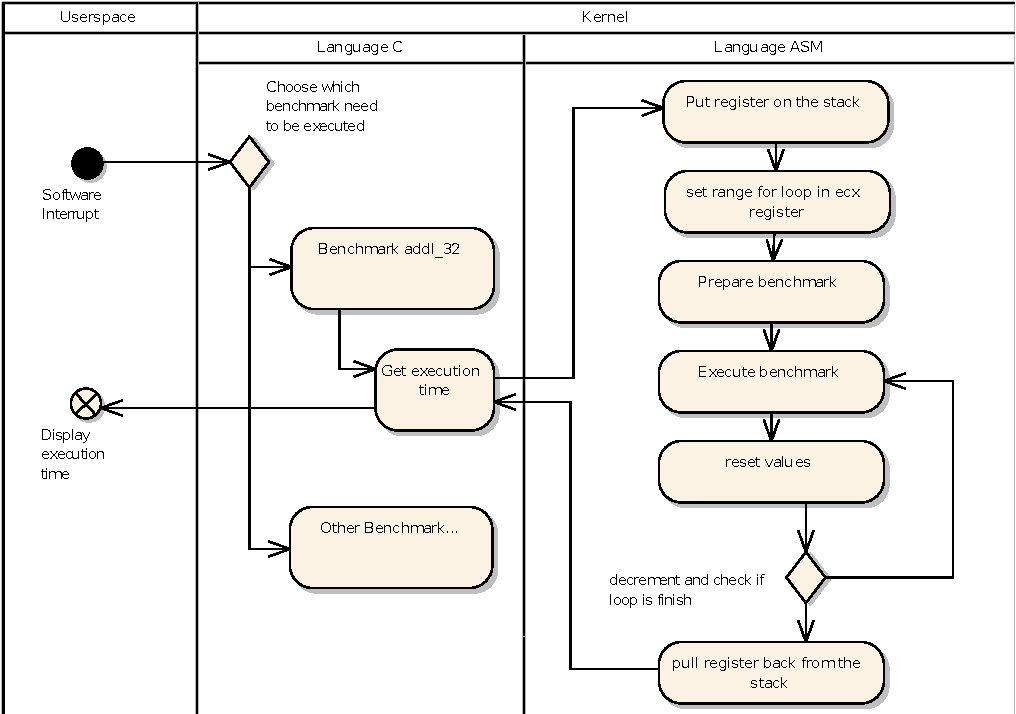
\includegraphics[scale=0.45]{images/interrupt_ea.pdf}
\caption{Interrupt}
\label{fig:Interrupt}
\end{wrapfigure}

Interrupts sind dafür gemacht, sofort verarbeitet zu werden. Ein kleines Beispiel soll dies veranschaulichen. Der Benutzer eines Computers drückt eine Taste auf der Tastatur. Dadurch produziert er ein Hardware-Interrupt. Der aktuelle Prozess wird gespeichert und angehalten. Der Kernel stellt über eine Vektor-Tabelle fest, um welchen Interrupt es sich handelt und führt die passende ISR aus, die zur Verarbeitung der gedrückten Tasten dient. Die ISR besteht aus einem sehr kurzem Programmcode (Microcode). In diesem Fall speichert der Programmcode die gedrückte Taste im RAM und gibt die Ressourcen wieder frei. Der letzte Prozess wird danach, falls er nicht bereits beendet war, weitergeführt. Die Interrupts sind nötig, um die Daten im Zeitpunkt des Geschehens zu verarbeiten.
\par

\autoref{fig:Interrupt} stellt die unterschiedlichen Interrupts und den Ablauf nach einem eingehenden Interrupt dar. Die Hardware-Interrupts\footnote{Je nach Literatur, Sprache oder Betriebssystem werden unterschiedliche Fachausdrücke verwendet. Der Kontext bleibt aber derselbe.} wurden bereits oben beschrieben. Die "Exception / Trap" sind Interrupts, die die CPU selber produziert. Ein Beispiel für ein solches Interrupt ist "Divisions by Zero". Dabei probiert man, eine Zahl durch Null zu teilen. Die Messmethode in dieser Arbeit stützt sich auf Software-Interrupts. Software-Interrupts werden als Systemcall bezeichnet, die häufig verwendet werden, um durch einen Kontextwechsel eine Aufgabe dem Kernel zu übergeben. Beim Kontextwechsel wird vom unprivilegierten Ring (Benutzermodus) in den privilegierten Ring (Kernelmodus) gewechselt. Dadurch kann auf Befehlssätze und Speicheradressen zugegriffen werden, was im Benutzermodus nicht möglich wäre, ohne unsicheren Code ausführen zu müssen. Systemcalls werden als ISR im selben Kontext ausgeführt wie Interrupts.




\section{Starten des Benchmarks über procfs}

Der Benchmark wurde in Form eines Kernelmoduls für ein Linux Betriebssystem gebaut. Das Kernelmodul registriert für jeden Benchmark ein Pseudofile, das unter der Verzeichnisstruktur \texttt{/proc/benchmark/} abrufbar ist.
\par
Das \texttt{procfs} oder \texttt{proc filesystem} genannte Filesystem erstellt eine Schnittstelle zwischen dem Benutzermodus und dem Kernelmodus. Es ist ein virtuelles Filesystem, das unter der Verzeichnisstruktur \texttt{/proc} gemountet wird\cite{mauerer2010professional}. Die Dateien, die sich darin befinden, sind Pseudofiles. Sie sind virtuell, weil sie nicht physisch existieren und somit auch nicht auf ein Medium gespeichert werden können. Beim Schreiben beziehungsweise Lesen der Pseudofiles werden die Informationen dem Kernel weitergegeben, verarbeitet und die Informationen werden zum Lesen im Benutzermodus bereitgestellt. Weil das Verhalten der Schnittstelle den Eigenschaften einer Datei entspricht, können für die Lese- und Schreiboperationen die Linux-Standardwerkzeuge verwendet werden.

\lstset{language=bash}
\begin{minipage}{\linewidth}
\begin{lstlisting}[label={list:read_procfs},caption={Lesen im procfs}]
sriolo@desktop ~ $ cat /proc/uptime 
571433.06 1229766.89
\end{lstlisting}
\begin{lstlisting}[label={list:write_procfs},caption={Schreiben im procfs}]
sriolo@desktop ~ $ echo 1 > /proc/sys/net/ipv4/conf/default/forwarding
\end{lstlisting}
\end{minipage}


Im ersten Beispiel \autoref{list:read_procfs} wird aus der Datei \texttt{uptime} gelesen. Dabei wird durch einen Systemcall die Betriebszeit berechnet und zurückgegeben. Das folgende, zweite Beispiel \autoref{list:write_procfs} zeigt, wie in einer Datei geschrieben werden kann. Dabei wird dem Kernel mitgeteilt, dass er das IP-Forwarding einschalten soll. Einen ähnlichen Aufbau hat das \texttt{sys filesystem}. Die Kommunikation ist dabei schwieriger, weil das Design für Menschen nicht lesbar ist, sondern lediglich für Programme im Benutzermodus. Im Gegensatz dazu kann das \texttt{procfs} mit den Standard-Werkzeugen im ASCII-Format gelesen und geschrieben werden.
\par
Das \texttt{procfs} ist an dieser Stelle wichtig, weil der Benchmark im Kernelmodus laufen muss. Durch den Befehl \texttt{cat} auf die entsprechende Datei des Benchmarks startet im Kernelmodus der Ablauf für die Messung und gibt die verwendete Zeit als Ausgabe an. Das folgende Beispiel in der \autoref{list:start_benchmark} veranschaulicht, wie der Benchmark gestartet und die CPU durch eine Addieroperation ausgelastet wird.

\lstset{language=bash}
\begin{minipage}{\linewidth}
\begin{lstlisting}[label={list:start_benchmark},caption={Starten des Benchmarks}]
root@galileo ~ $ cat /proc/benchmark/addl_32
321
\end{lstlisting}
\end{minipage}


\section{Aufbau der Software für die Messung}


\subsection{Grundaufbau und Ablauf eines Benchmarks}
Der Grundbau der Software wurde mit der Programmiersprache C geschrieben. Der Kern des Benchmarks besteht aus wenigen Assembler-Befehlssätzen. Das Kernelmodul beinhaltet alle für diese Arbeit relevanten Benchmarks. Die \autoref{fig:Benchmark} stellt den Ablauf des Programms dar.

\begin{figure}[H]
\centering
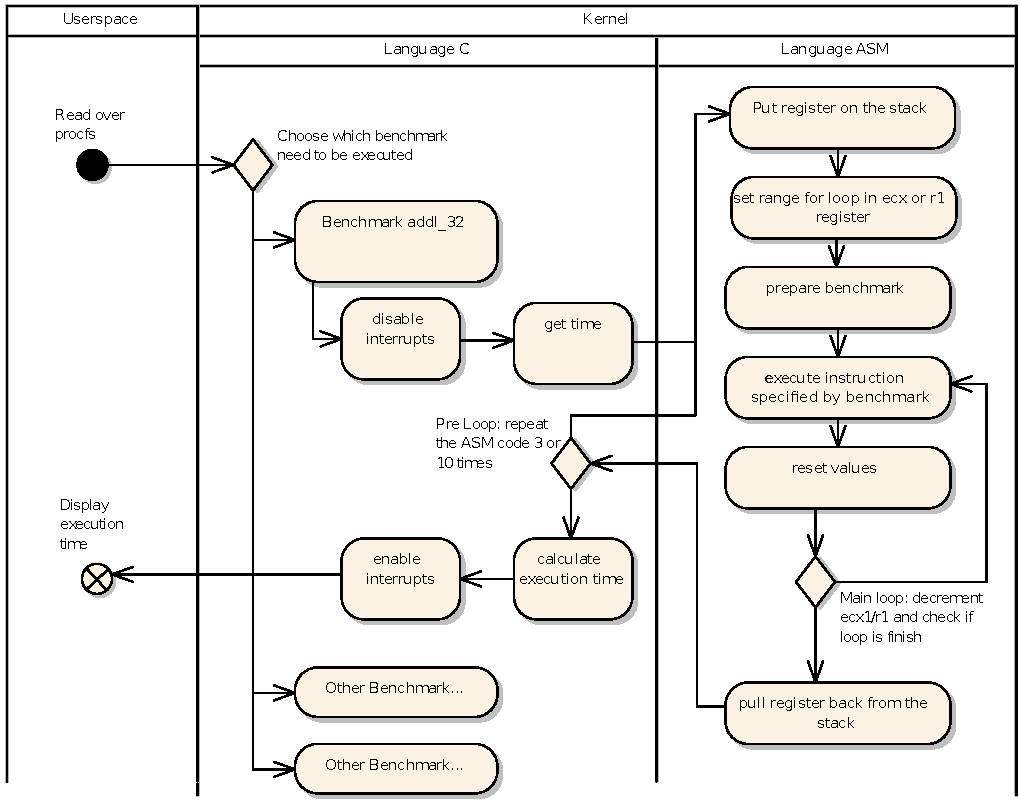
\includegraphics[width=1.0\textwidth]{images/benchmark_ea.pdf}
\caption{Benchmark}
\label{fig:Benchmark}
\end{figure}


Durch einen Systemcall, der über das \texttt{procfs} ausgelöst wird, wird der Benchmark gestartet. Da sich in der Software mehrere Benchmarks befinden, muss zuerst einer dieser Benchmarks ermittelt werden. An dieser Stelle werden durch die Funktion \texttt{local\_irq\_save} alle weiteren Interrupts geblockt. Die Startzeit wird eruiert und zwischengespeichert. Das Programm wechselt zum eigentlichen Benchmark, der in Assembler geschrieben ist. Ist der Assembler-Teil abgearbeitet, wird die Zeit errechnet, die zur Durchführung des Benchmarks verwendet worden ist. Durch den Aufruf der Funktion \texttt{local\_irq\_restore} wird die Blockierung von weiteren Interrupts wieder aufgehoben. Als letztes wird die vom Benchmark aufgewendete Zeit in den Systemcall zurückgeliefert.
\par
Die Grösse der Schleife, die in Assembler geschrieben worden ist, ist auf die Anzahl ihrer möglichen Wiederholungen beschränkt. Beide Boards haben eine 32bit-Architektur. Die maximale Anzahl der Durchläufe kann somit die Wortbreite von 32bit grundsätzlich nicht übersteigen. Damit die Messung eines Benchmarks dennoch über einen längeren Zeitraum gemessen werden kann, wird ein einfacher Trick angewendet. Um den Assembler-Code wird eine Vorschleife gelegt. Diese Vorschleife verlängert die Ausführung des Benchmarks um das drei- bis zehnfache. Die genaue Anzahl der Durchgänge pro Board ist aus \autoref{fig:benchmark_loop_size} ersichtlich. Die Auswirkungen der Vorschleife auf das Messresultat sind gering, da die Vorschleife um ein x-faches kleiner ist als die Endschleife. Demzufolge beeinflusst sie das Ergebnis kaum und ist dementsprechend vernachlässigbar.

\begin{figure}[H]
\center
\begin{tabular}{ |l|l|l|l| }
\hline
Board & Vorschleife (C) & Endschleife (Assembler) & Total \\ \hhline{|=|=|=|=|}
Galileo & 3 & 2147483648 & $\approx$6.4 Mrd.  \\ \hline
Raspberry Pi & 10 & 2147483648 & $\approx$21.4 Mrd. \\ \hline
\end{tabular}
\caption{Anzahl Durchläufe eines zu testenden Befehlssatzes}
\label{fig:benchmark_loop_size}
\end{figure}



\begin{minipage}{\linewidth}
\lstset{language=[x64]Assembler}
\begin{lstlisting}[label={list:asm_benchmark},caption={Benchmark in Assembler}]
benchmark_imull_zero:
  stmfd    sp!, {r0-r5}
  ldr r1, = 2147483648
  ldr r3, = 0x0
  ldr r4, = 0x0
loop_benchmark_imull_zero:
  mul r5, r3, r4
  sub r1, r1, #1
  cmp r1, #0
  bge loop_benchmark_imull_zero
  ldmfd    sp!, {r0-r5}
  bx  lr
\end{lstlisting}
\end{minipage}


In der \autoref{list:asm_benchmark} ist der Assemblercode aufgeführt, der die CPU über einen längeren Zeitraum mit der Rechenoperation $0*0$ stresst. Die \autoref{list:asm_benchmark} dient als Beispiel für die Grundstruktur eines Benchmarks. Auf dieser basieren dann die unterschiedlichen Benchmarks, die je einen Befehlssatz beinhalten, der mit den anderen verglichen werden kann. Der Prozessor startet bei Zeile 1 und im nächsten Schritt werden alle Register \texttt{r1} bis \texttt{r5} im RAM auf einen Stack gelegt. Das Register \texttt{r1} wird mit $2^{31}$ gefüllt. Dieses dient dazu, später eine Schlaufe zu erzeugen. In Zeile 4 und 5 wird der Benchmark auf die Rechenoperation vorbereitet, wobei \texttt{r3} und \texttt{r4} auf null gesetzt werden. Der Prozessor wechselt nun zur wichtigsten Zeile, der Nummer 7. An dieser Stelle befindet sich die Multiplikationsoperation, die eine Veränderung des Energieverbrauchs erzeugt und diesen misst. Nach der Abarbeitung wird der Index im Register \texttt{r1} um eins dekrementiert. Anschliessend wird überprüft, ob der Index bereits null erreicht hat. Falls der Index noch nicht auf null ist, wird ein Programmsprung auf Zeile 7 erzeugt und die Schleife noch einmal wiederholt. Falls der Index null erreicht hat, wird der Programmsprung nicht erzeugt und dies führt zum Austritt aus der Schleife. Die Register \texttt{r1} bis \texttt{r5}, die am Anfang auf den Stack gelegt wurden, werden aus dem RAM geholt und wiederhergestellt. Damit ist das Assemblerprogramm zu Ende.
\par
In der \autoref{list:asm_benchmark} ist erkennbar, dass mehrere Befehlssätze erforderlich sind, um eine Schleife zu erstellen. Obwohl nur die Zeile 7 für den Benchmark relevant ist, müssen die Zeilen 8, 9 sowie 10 zwangsläufig programmiert werden und verfälschen das Messresultat. Damit ein aussagekräftiger Vergleich zwischen unterschiedlichen Benchmarks erstellt werden kann, muss die Grundstruktur daher immer gleich sein. Somit ist die Messung zwar nicht korrekt, da es sich jedoch immer um den gleichen Fehler handelt, können Vergleiche zwischen den Benchmarks gezogen werden.

\pagebreak
\subsection{Kompilation und Programmstruktur}

\begin{wrapfigure}{!}{0.7\textwidth}
\centering
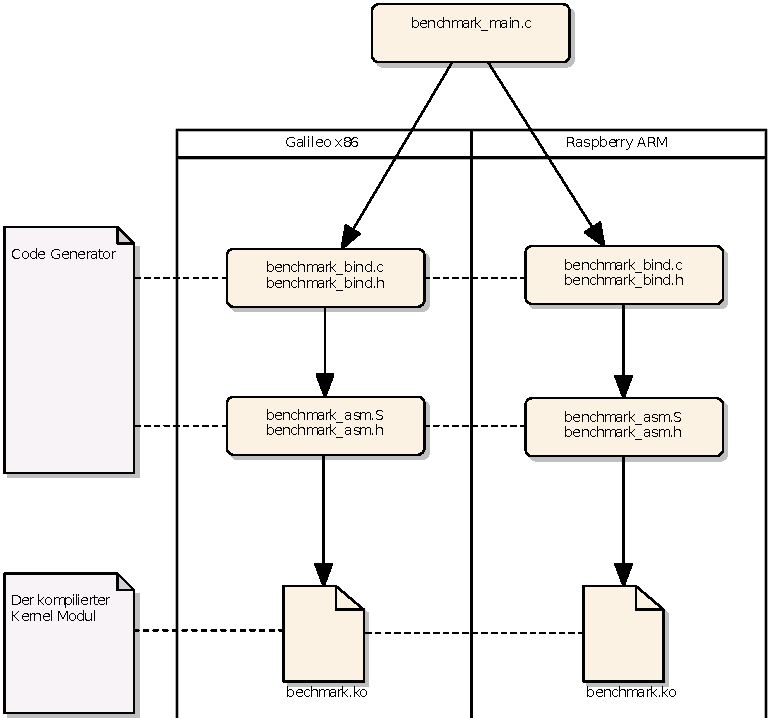
\includegraphics[scale=0.7]{images/filestructure.pdf}
\caption{Dateistruktur}
\label{fig:filestructure}
\end{wrapfigure}


Da die Grundstruktur des Benchmarks für jede Messung immer gleich ist, wurde ein Code-Generator in Python geschrieben. Dieser erstellt für jeden Benchmark automatisch die Grundstruktur und übernimmt den Inhalt aus einer Konfigurationsdatei. Der Code-Generator wird vor dem Kompilieren automatisch gestartet. Die Dateien werden an den richtigen Ort geschrieben, damit sie der GCC kompilieren und anschliessend mit dem Kernelmodul verlinken kann. Die Grundstruktur des Kernelmoduls liegt in der Datei \texttt{benchmark\_main.c}. Die Datei \texttt{benchmark\_bind.c} sorgt für den Übergang von C in Assemblercode, der sich in der Datei \texttt{benchmark\_asm.S} befindet.
\par
Der Kompiliervorgang dauert auf einem SoC zu lange, weil der Prozessor zu schwach ist. Deshalb wurde das Kernelmodul für die SoCs auf eine leistungstarke Maschine kompiliert. Wenn Sourcecode auf einer Maschine für eine andere Maschine kompiliert wird, heisst dieser Vorgang cross-kompilieren. Wird nun während dieses Vorgangs ein Kernelmodul kompiliert, muss der Kompiler die Headerfiles des Kernels, in den das Kernelmodul später eingefügt wird, kennen. Zusätzlich enthält nicht jede Linux-Distribution Headerfiles. Dies gilt hier sowohl für das Raspberry Pi-, als auch für das Galileo-Board. Vor der Kompilation müssen deshalb die passenden Kernels, welche ihrerseits Headerfiles beinhalten, auf der leistungsstarke Maschine erbaut werden. Nur so ist eine erfolgreiche Kompilation durchführbar. Beim Raspberry Pi-Board wird noch zusätzlich ein modifizierter GCC benötigt, der vor der Kompilation installiert werden muss. Dieser steht auf der offiziellen Seite von Raspberry Pi zum Download bereit. Die technische Dokumentation findet sich im Wiki meines Projektes zur Thesis unter \url{https://github.com/codeix/thesis_ffhs_2016/wiki}. Auf der gleichen Plattform stehen auch alle erforderlichen Dateien zur Nachvollziehbarkeit des Experiments zum Download bereit (ca. 800MB). Nach dem fehlerfreien Kompilieren des Kernelmoduls kann dieses auf das Board kopiert und mit dem Befehl \texttt{insmod} in den Kernel geladen werden.


